\documentclass{tfgitic}[2024/07/01]
% « »
% Aqui carregueu packages complementaris que necessiteu
\usepackage{biblatex}
% \usepackage[table,xcdraw]{xcolor}
\usepackage{colortbl}
\usepackage{booktabs}
\usepackage{hhline}
\usepackage{caption}

\usepackage{bytefield}

\usepackage{tikz}
\usetikzlibrary{arrows.meta, positioning, calc, decorations.markings}

\renewcommand{\figureautorefname}{figura}
\renewcommand{\tableautorefname}{taula}
\renewcommand{\sectionautorefname}{secció}
\renewcommand{\subsectionautorefname}{apartat}
\renewcommand{\subsubsectionautorefname}{subapartat}
\renewcommand{\chapterautorefname}{capítol}


\tikzset{
  cross at end/.style={
    postaction={
      decorate,
      decoration={
        markings,
        mark=at position 1 with {
          \draw[solid, line width=0.6pt, color=black]
            (-2pt,-2pt) -- (2pt,2pt)
            (-2pt,2pt) -- (2pt,-2pt);
        }
      }
    }
  }
}

% Indica quines bd bibliografiques usarem
\addbibresource{tfe.bib}

% \title{Disseny d’un protocol LoRa amb encaminament estàtic per aplicacions de monitoratge}
\title{Disseny d’un protocol LoRa amb encaminament estàtic per aplicacions de monitoratge}
\subtitle{Aplicació en xarxes de baix consum mitjançant sincronització temporal}
% \subtitle{Adaptació per a escenaris de baix consum mitjançant sincronització temporal}

% L'autor del treball. Admet gènere (vegeu 9.2 del manual) fent \author[f]{}
\author{Pol Flotats Sabata}

% La direcció. Un treball ordinari te un o excepcionalment dos directors.
% admet gènerer i número (vegeu 9.2 del manual)
\advisor{Jordi Bonet Dalmau i Arnau Arumi Casanovas}

% Si el treball es fa sota un conveni de pràctiques (modalitat empresa)
% llavors el director (advisor) és la persona de la empresa que
% dirigeix el treball i, a més, hi ha un professor que fa de tutor (counselor).
% En aquest cas també es consigna l'empresa (company)
% \counselor admet gènere (vegeu 9.2 del manual)
%
% \counselor{}
% \company{}

% Els àmbits temàtics en que es classifica el treball. Pregunteu al
% director.
\topics{}

% Si voleu dedicatòria descomenteu
%\dedication{}

% Si voleu agraïments descomenteu
%\begin{acknowledgments}
%\end{acknowledgments}


\begin{resum}
\end{resum}

\begin{abstract}
\end{abstract}




\begin{document}

% Si feu servir apèndixs, descomenteu
%\part{Memòria}

\chapter{Introducció}
\section{Objectius}
\section{Limitacions i abast del treball}
\section{Estructura de la memòria}
% primera part on es fa disseny d'un protocol genèric i NO centrat en baix consum, sinó en generalització i nodes amb taules estàtiques
% segona part on es fa un disseny centrat en baix consum i sincronització temporal

\chapter{Antecedents}
\section{Protocols de comunicació: capes i modularitat}
\label{sec:protocols}
Un protocol de comunicació defineix com dos o més dispositius d'una xarxa poden intercanviar informació. Ho fa mitjançant regles i normes que determinen la sintaxi ---format dels missatges---, la semàntica ---el seu significat---, i mecanismes de detecció i correcció d'errors.

Per tal que es pugui establir una comunicació, és necessari que els dispositius involucrats implementin el mateix protocol. Per facilitar-ho, es defineixen estàndards tècnics, publicats per organitzacions com l'\acro{iso} o l'\acro{ieee}, permetent que els fabricants puguin dissenyar dispositius compatibles. Un exemple de protocol estandaritzat és \acro{http}, amb el seu detall consultable a \cite{fielding_hypertext_2014}.

Per facilitar el disseny i implementació dels protocols, sovint es descomposen en protocols més simples. Aquests es poden agrupar en capes, on cada capa s'encarrega d'una part específica del procés de comunicació. El resultat és el que es coneix com una pila de protocols. 
En aquests dissenys, cada capa depèn de les capes inferiors per realitzar les seves funcions, i proporciona serveis a les capes superiors. El disseny i verificació de cada capa es pot fer de forma independent, i ofereixen la possibilitat d'implementar diferents protocols en cada capa, sempre que es mantingui la interfície definida entre elles.

Un dels models més coneguts és el model \acro{osi}, definit per set capes. Tot i no ser utilitzat en sistemes reals, és de gran utilitat en entorns acadèmics per comprendre la divisió per capes. Per a més informació, es pot consultar \cite{noauthor_isoiec_1994}.

En sistemes reals, el model més utilitzat és el model \acro{tcp/ip}, que estableix les bases d'Internet. Està format per quatre capes:
\begin{enumerate}
    \item \emph{Enllaç}. És la capa de més baix nivell. S'encarrega de la comunicació entre dispositius d'una mateixa xarxa ---és a dir, es poden comunicar directament---, i de la detecció i correció d'errors produits en la comunicació. També gestiona l'accés al medi físic per on es transmeten les dades, que sovint és compartit amb altres dispositius.
    \item \emph{Xarxa}. Gestiona la comunicació entre dispositius que es troben en xarxes diferents i, per tant, no es poden comunicar directament. Per fer-ho, s'utilitzen dispositius intermedis, coneguts com a encaminadors (\est{routers}), que determinen la ruta més eficient per fer arribar les dades al seu destí.
    \item \emph{Transport}. Defineix la connexió d'extrem a extrem entre els dispositius origen i destí i, si és necessari, que la transmissió sigui fiable. Els protocols d'aquesta capa poden oferir mecanismes com l'ordenació de missatges, l'eliminació de missatges duplicats i la gestió de congestió. Els dos protocols més coneguts d'aquesta capa són \acro{tcp}, que garanteix la transmissió fiable de dades mitjançant confirmacions i retransmissions, i \acro{udp}, que no garanteix fiabilitat, però és més eficient per aplicacions en temps real com el contingut en estríming o videjocs.
    \item \emph{Aplicació}. És la capa més alta i propera a l'usuari final. Defineix els protocols que utilitzen les aplicacions per comunicar-se a través de la xarxa, com ara \acro{http}, utilitzat per a la navegació web, o protocols de suport, com ara \acro{dns}, per a la resolució de noms de domini.
\end{enumerate}
Per a l'estàndard complet i més detall, es pot consultar \cite{braden_requirements_1989}. 

% \subsection{Referència al model TCP/IP}
\section{Tecnologia LoRa i LoRaWAN}
Els termes \emph{LoRa} i \emph{LoRaWAN} sovint es confonen i s'utilitzen ambdós termes indistintament. Mentre que el primer és una tecnologia propietària, el segon és mantingut per una associació sense ànim de lucre. En aquest apartat es presenten ambdues tecnologies, indicant-ne les seves característiques i limitacions.

\subsection{LoRa}
% TODO: Explicar estructura missatge LoRa? Preambul?
% Mencionar mida màxima de les dades?
El nom de \emph{LoRa} prové de l'anglès \est{Long Range}. És una tecnologia de comunicació sense fils, de llarg abast, i de baix consum, fent que sigui especialment útil per a aplicacions d'Internet de les Coses (\acro{iot}). Va ser desenvolupada per \emph{Cycleo}, que va ser adquirida per \emph{Semtech} el 2012.

Utilitza freqüència sub-GHz en bandes \acro{ism} ---\emph{Industrial, Scientific and Medical}---, que són bandes de freqüència lliures de llicència. Això permet que qualsevol persona pugui utilitzar la tecnologia sense necessitat d'obtenir una llicència. Malgrat això, existeixen limitacions legals, com la potència màxima de transmissió o la quantitat de dades que es poden transmetre en un període de temps determinat. Per a més informació, es pot consultar \ref{subsec:limitacions_legals}.

Per assolir una comunicació de llarg abast, LoRa utilitza modulació de \emph{chirp spread spectrum} (\acro{css}), que permet una comunicació robusta i fiable en entorns amb interferències. Aquesta modulació es basa en codificar cada símbol com un senyal que s'escampa per tot l'ample de banda disponible, augmentant (o disminuint) de forma lineal la freqüència al llarg del temps. Gràcies a que la freqüència varia de forma lineal, també és resistent a l'efecte \emph{Doppler}, com s'ha estudiat a \cite{doroshkin_experimental_2019}. Una representació visual del funcionament de la modulació \acro{css} es pot veure a \cite{richard_wenner_lora_2017}.

Consta de diversos paràmetres que es poden ajustar per adaptar la comunicació a diferents necessitats:
\begin{itemize}
    \item \emph{Ample de banda}. És l'ample de banda (\acro{bw}) del canal de transmissió, sovint de \SI{125}{\kHz}, però també pot ser de \SI{250}{\kHz} o \SI{500}{\kHz}. Un ample de banda més gran permet una major velocitat de transmissió, però redueix la sensibilitat de recepció i, per tant, el rang de comunicació.
    \item \emph{Data rate}. És la velocitat de transmissió de dades (\acro{dr}), que depèn de l'ample de banda i del factor d'espargiment. Un data rate més alt permet una major velocitat de transmissió, però redueix la sensibilitat de recepció i, per tant, el rang de comunicació.
    \item \emph{Spreading Factor}. El factor d'espargiment (\acro{sf}) defineix la durada dels símbols i, per tant, la velocitat de transmissió. Es correspon amb la quantitat de bits d'informació que codifica cada símbol. Un \acro{sf} més alt permet una major sensibilitat de recepció, ja que cada símbol ocupa més temps i, per tant, és més fàcil de detectar. Això permet una comunicació a llarg abast, però redueix la velocitat de transmissió. Els valors possibles de \acro{sf} són entre 7 i 12 i, per cada increment de 1 d'\acro{sf}, es redueix la velocitat de transmissió a la meitat. Una característica molt important és que els diferents \acro{sf} són ortogonals entre ells. Això implica que senyals modulats amb diferents \acro{sf} i en un mateix canal no interfereixin entre ells. 
    \item \emph{Coding Rate}. La taxa de codificació (\acro{cr}) defineix la proporció d'informació útil que es transmet en comparació amb la quantitat total de dades enviades. Els possibles valors són $\frac{4}{5}$, $\frac{4}{6}$, $\frac{4}{7}$ i $\frac{4}{8}$. Així, per un \acro{cr} de $\frac{4}{5}$, per cada quatre bits d'informació útil, se n'afegeix un de redundància.
\end{itemize}

Tots aquests paràmetres estan relacionats entre ells, i és important trobar un equilibri entre ells per aconseguir la millor comunicació possible. Per exemple, si es vol obtenir una comunicació a llarg abast, es pot augmentar el \acro{sf} i el \acro{cr}. Això reduirà la velocitat de transmissió i, per tant, augmentarà el consum energètic, ja que serà necessari estar transmetent més temps. En canvi, si es vol una comunicació ràpida, es pot reduir el \acro{sf} i augmentar el \acro{bw}, però això reduirà el rang de comunicació.

Amb una configuració adequada, es poden aconseguir comunicacions de fins a quinze quilòmetres en entorns rurals, i amb una vida útil de les bateries de diversos mesos i anys, com especifica Semtech a \cite{noauthor_lora_2024}.

Per tal que el transmissor i el receptor es puguin sincronitzar, LoRa utilitza un preàmbul de sincronització. Aquest preàmbul és un senyal de referència que permet al receptor detectar l'inici d'una transmissió i sincronitzar-se amb el transmissor. La durada del preàmbul és configurable, però sovint s'estableix de vuit símbols. Una durada major ofereix més garenties que el receptor pugui detectar la transmissió, però augmenta el temps total de transmissió i, per tant, el consum energètic.

Després de transmetre el preàmbul, es transmeten les dades del missatge. Un fet a tenir en compte és que, ja que està pensat per a ser utilitzat en dispositius de baix consum, i a la baixa velocitat de transmissió, la quantitat màxima de dades que molts transductors permeten enviar és de \SI{255}{\byte}.

Per assegurar la integritat de les dades rebudes, LoRa ofereix la possibilitat d'incloure un codi de detecció d'errors (\acro{crc}). Aquest codi es calcula a partir de les dades del missatge i s'afegeix al final del missatge. El receptor pot utilitzar aquest codi per verificar si les dades rebudes són correctes. Si el codi no coincideix amb les dades rebudes, el receptor pot descartar el missatge.


\subsection{LoRaWAN}
% TODO: QUEDA EXPLICAR JOIN (OTAA I ABP)
Pel que fa a LoRaWAN, es tracta d'una definició de l'arquitectura d'un sistema \acro{LPWAN} (\est{Low Power Wide Area Network}), desenvolupada i mantenida per la \href{https://lora-alliance.org}{LoRa Alliance}. Defineix el protocol de comunicació i l'arquitectura de la xarxa, així com els mecanismes de seguretat i gestió de la xarxa. 

Utilitzant l'estructura per capes vista a la \autoref{sec:protocols}, LoRaWAN opera principalment a nivell d'enllaç, malgrat que també implementa característiques d'altres capes (com ara el control de sessions). A nivell físic, utilitza la modulació LoRa.

Pel que fa a l'estructura de la xarxa, consta de 4 components principals:
\begin{itemize}
    \item \emph{Dispositius finals}. Sensors o actuadors que transmeten, a través de LoRa, missatges als \est{gateways}, conegut com a \est{uplinks}. També pot ser a l'inrevés, on els \est{gateways} transmeten missatges als dispositius finals, conegut com a \est{downlinks}.  
    \item \emph{Gateways}. Dispositius que reben els missatges dels dispositius finals i els transmeten al servidor de la xarxa. La comunicació entre els \est{gateways} i el servidor de la xarxa es realitza a través d'Internet, i no utilitza LoRa. 
    \item \emph{Servidor de la xarxa}. Dispositiu que gestiona els dispositius finals, els \est{gateways} i aplicacions de la xarxa. S'encarrega de la gestió de les comunicacions, la seguretat i la configuració dels dispositius finals. Gestionen també el xifrat punt a punt ---entre dispositius finals i servidors d'aplicació---.
    \item \emph{Servidor d'aplicació}. Processa les dades d'aplicació enviades pels dispositius finals.
\end{itemize}
Aquests dispositius es troben organitzats en una estructura d'«estrella d'estrelles», on a la part central hi trobem el servidor de la xarxa. Aquest es comunica amb múltiples \est{gateways}, i cada \est{gateway} es comunica a la vegada amb múltiples dispositius finals. 
Un fet important és que un dispositiu final no escull el \est{gateway} amb qui comunicar-se: en transmetre, tots els \est{gateways} que reben les dades ho reenvien al servidor de la xarxa. El servidor de xarxa és qui s'encarrega de detecar missatges duplicats i escollir quin és el millor \est{gateway} per transmetre un \est{downlink}. Aquesta estructura simplifica el disseny dels dispositius finals, amb el cost d'una major complexitat en el servidor de xarxa, tenint en compte que hi ha un únic servidor de xarxa per una quantitat N de dispositius finals.

Els dispositius finals poden operar en tres modes diferents, coneguts com a \emph{classes}:
\begin{itemize}
    \item \emph{Classe A}. És la classe més senzilla i de menor consum. Els dispositius finals només poden rebre missatges després d'haver realitzat una transmissió (\est{uplink}), moment en el qual obren dues finestres de recepció per rebre \est{downlinks}. Aquesta és la classe més utilitzada en aplicacions d'\acro{iot}, ja que permet un funcionament de baix consum, sent únicament necessari posar-se en mode de recepció després de fer una transmissió.
    \item \emph{Classe B}. Els dispositius finals obren finestres de recepció en moments predeterminats (coneguts com a \est{ping slots}), a més de les finestres de recepció que obren després d'un \est{uplink}. Aquest fet fa que la latència de recepció de \est{downlinks} sigui molt menor que en la classe A.
    \item \emph{Classe C}. Obren també dues finestres de recepció després d'un \est{uplink}, amb la diferència que la segona finestra es manté oberta fins la següent transmissió. Així, es pot considerar que aquests dispositius sempre estan rebent, amb l'exepció de quan transmeten. La latència de recepció de \est{downlinks} és la mínima d'entre les tres classes, però el consum energètic és màxim.
\end{itemize}

Una altra característica important de LoRaWAN és la seva capacitat d'autoajustament, conegut com a \acro{adr} (\est{Adaptative Data Rate}). Els dispositius finals poden ajustar automàticament els paràmetres de comunicació, com el \acro{sf} o la potència de transmissió, per adaptar-se a les condicions del canal de comunicació. Quan s'utilitza, el servidor de la xarxa pot indicar als dispositius finals quins paràmetres utilitzar, reduint el consum energètic i possibles interferències amb altres dispositius. Per exemple, un dispositiu molt proper a un \est{gateway} hauria d'utilitzar \acro{sf} més baixos, mentre que dispositius llunyans n'haurien d'utilitzar de més elevats.

\subsection{The Things Network}
Es tracta d'un projecte d'\acro{iot} que proporciona un servidor de xarxa públic i gratuït. El seu objectiu és crear una xarxa global de dispositius LoRaWAN, permetent la comunicació entre ells sense necessitat d'infraestructura pròpia. Els usuaris poden connectar els seus \est{gateways} a la xarxa i compartir la seva cobertura amb altres usuaris.

També ofereix la possibilitat d'afegir dispositius finals a la xarxa, i gestionar-los a través de la seva interfície web. A més, permeten la integració amb altres serveis, com ara \emph{Node-RED} o \emph{Grafana}, per visualitzar i analitzar les dades dels dispositius finals.

\subsection{Limitacions legals}
\label{subsec:limitacions_legals}
Com s'ha comentat anteriorment, LoRa utilitza bandes de freqüència lliures de llicència. Per garantir un ús adequat d'aquestes bandes, cada país estableix una sèrie de limitacions legals. Aquestes limitacions poden variar d'un país a un altre, i és important tenir-les en compte a l'hora de dissenyar un sistema de comunicació LoRa. 

Pel que fa a la Unió Europea, l'entitat responsable de la regulació de les comunicacions és l'\acro{etsi} (\est{European Telecommunications Standards Institute}). Estableix l'ús de LoRa en les freqüències entre \SI{863}{\MHz} i \SI{870}{\MHz}, amb un ample de banda màxim de \SI{250}{\kHz}.

A més, estableix un límit de potència màxima de transmissió, i un màxim d'utilització del canal. Aquestes limitacions depenen de la sub-banda utilitzada (dins el rang anteriorment mencionat), però de forma genèrica es considera una potència màxima de \SI{16}{\deci\bel\text{m}}, i una utilització màxima del canal (conegut com a \emph{duty cyle}) de l'\SI{1}{\%}. Així, per cada hora de funcionament, poden transmetre un màxim de 36 segons. Tots els detalls sobre les limitacions legals a la Unió Europea es poden consultar a \cite{etsi_etsi_nodate}.

Si s'utilitza un servidor de xarxa públic com \emph{The Things Network}, és important tenir en compte que aquest també pot aplicar limitacions addicionals. Pel que fa a \acro{ttn}, estableix una política d'ús just (\emph{fair use policy}) que limita l'ús del canal en 30 segons per dispositiu final i dia. A més, s'estableix un límit de deu \est{downlinks} per dispositiu i dia. És important tenir aquestes limitacions en compte en dissenyar un sistema; en cas d'incumpliment, el servidor de xarxa podria bloquejar l'accés del dispositiu final.

\section{Treballs relacionats}
\label{sec:treballs_relacionats}
Existeixen diversos projectes amb un objectiu similar al d'aquest treball, com ara \emph{Meshtastic} o \emph{LoRaMesher}. Tots dos projectes utilitzen LoRa per crear xarxes de comunicació entre dispositius finals, però presenten diferencies amb els objectius d'aquest treball. A més, consten també de limitacions, a les qual se'ls vol donar solució. En aquest apartat es presenten ambdós projectes, amb les seves característiques i limitacions, així com diferències vers el treball presentat. 

\subsection{Meshtastic}
Es tracta d'un projecte de codi obert que té com a objectiu crear una xarxa de comunicació descentralitzada, i pensada per a ser utilitzada en dispositius de baix consum i cost. El seu repositori es troba disponible a \href{https://github.com/meshtastic}{GitHub}.

Utilitza comunicació LoRa per a transmetre missatges entre dispositius, evitant dependre d'altres infraestructures com internet. Per tal d'aconseguir-ho, tots els dispositius actuen com a encaminadors: quan reben un missatge que no està destinat a ells, el reenvien, permetent que altres dispositius puguin repetir l'encaminament fins arribar al destí final. Una característica molt interessant d'aquest projecte és que ofereix aplicacions mòbils i web per interactuar amb els dispositius de la xarxa, permetent enviar missatges de forma molt senzilla.

L'estratègia d'encaminament que utilitza es basa en «inundació» (\est{flooding}), on cada dispositiu reenvia tots els missatges que rep, sempre que no sigui ell el destinetari, sense tenir en compte si ja els ha rebut o no. Aquest disseny tampoc considera la ubicació del destí final, fent que el missatge es transmeti per tota la xarxa. Aquests fets poden provocar un sobreús del canal, i un augment del consum energètic dels dispositius. 

Per intentar reduir aquest efecte, implementa un estil d'«inundació controlada». Quan un dispositiu rep un missatge, espera un temps proporcional a la relació senyal soroll (\acro{snr}) del missatge rebut abans de retransmetre, i cance\l.la l'enviament si un node realitza la transmissió abans. Així, un dispositiu més proper a l'origen (major \acro{snr}) esperarà més temps que un de llunyà i, per tant, el missatge el retransmetrà únicament el dispositiu llunyà. És cert que això redueix el nombre de transmissions que realitza cada dispositiu, però no evita que el missatge es retransmeti per tota la xarxa. 

Un altre inconvenient és que, a causa que els dispositius no saben quan altres dispositius realitzaran una transmissió, hagin d'estar sempre actius i en mode de recepció. Això provoca que el consum energètic dels dispositius sigui elevat (de l'ordre dels \SI{10}{\milli\watt}), fent-los poc adequats per aplicacions de monitoratge.

Durant el desenvolupament d'aquest treball, Meshtastic ha iniciat la implementació d'un protocol d'encaminament per a missatges entre dos únics dispositius. La idea d'aquest protocol és descobrir la ruta més òptima entre dos dispositius utilitzant el mecanisme d'«inundació controlada»; un cop el destí rep el missatge, respon amb un nou missatge amb la informació de la ruta, que conté tots els dispositius que han de retransmetre el missatge per arribar fins a ell. En el procés de fer arribar aquesta resposta al transmissor del missatge, tots els nodes intermedis poden generar la seva taula de rutes. En les següents transmissions, si es coneix la ruta, els missatges els reenvien únicament els nodes de la ruta. Els detalls de la implementació i funcionament d'aquest protocol es poden consultar a \cite{open_source_mesh_nodate}.

\section{LoRaMesher}
Es tracta d'una llibreria que implementa un protocol d'encaminament per a ser utilitzat en xarxes basades en LoRa. 

Cada dispositiu consta d'una taula d'encaminament, on es defineixen quin és el següent dispositiu a qui han d'enviar un missatge per fer-lo arribar al destí final. De forma periòdica, cada node transmet informació sobre la seva taula d'encaminament; els nodes que es troben a l'abast reben el missatge i actualitzen la seva taula d'encaminament amb la informació rebuda, no només coneixent informació sobre els seus veïns directes, sinó també sobre els veïns dels seus veïns, i així successivament. Es poden consultar els detalls d'aquesta implementació a \cite{sole_implementation_2022}.

Aquesta solució resol el problema de la «inundació controlada» presentat anteriorment, ja que únicament els nodes que es troben a la ruta reenvien el missatge. Malgrat això, presenta un dels inconvenients vists prèviament: tots els dispositius han d'estar sempre actius i en mode de recepció. Com s'ha mencionat, això provoca un consum elevat, reduint la viabilitat d'ús en aplicacions de monitoratge.

\chapter{Desenvolupament del protocol de comunicació}
En aquest capítol es presenta el disseny i implementació del protocol de comunicació. S'ha dissenyat amb l'objectiu de ser flexible, eficient, aplicable a una àmpla varietat de xarxes LoRa, i amb compatibilitat amb xarxes LoRaWAN. 

En un primer moment es fa un anàlisi de les característiques del protocol, així com la seva estructura. A continuació, es descriu l'entorn de desenvolupament i llibreries utilitzades. Seguidament, es presenta el disseny per capes del protocol, seguint l'estructura vista a la \autoref{sec:protocols}. Finalment, es mostra la implementació del protocol en un dispositiu real, i les verificacions realitzades per validar el funcionament.

No es farà especial menció a la implementació específica en codi de cada funcionalitat, si no que més bé es detallaran els criteris de disseny adoptats i les decisions preses. Es considera que, amb un disseny ben definit, la implementació del protocol és una tasca trivial. Malgrat això, es pot consultar la total del codi a \url{https://github.com/pfs26/Encaminament-LoRa/tree/main/firmware}.

\section{Característiques}
El disseny del protocol està fortament influenciat pel model \acro{tcp/ip}, presentat a la \autoref{sec:protocols}. El protocol presentat es basa en una pila de protocols, on cada capa s'encarrega d'una part específica del procés de comunicació. Això permet un disseny modular, i la possibilitat de modificar les funcionalitats d'una capa sense afectar la resta.

Es basa en una xarxa de dispositius estàtics, una característica habitual en sistemes de monitoratge. Aquest fet permet prescindir de mecanismes d'encaminament dinàmic, com els presentats a la \autoref{sec:treballs_relacionats}, ja que la xarxa no canvia amb el temps, permetent simplificar el protocol. Per altra banda, això implica que la topologia de la xarxa ha de ser dissenyada abans de la seva implementació, definint les taules d'encaminament de cada dispositiu.

En utilitzar la modulació LoRa, que com s'ha dit anteriorment utilitza freqüències \acro{ism}, intenta maximitzar l'eficiència d'ús del canal. Això redueix la generació d'interferències amb altres dispositius que utilitzin el mateix canal, el nombre de retransmissions, i un menor consum energètic.

Ofereix compatibilitat amb LoRaWAN, permetent que dispositius amb connexió a \est{gateways} puguin alternar entre l'ús del protocol dissenyat o LoRaWAN. Això ofereix la possibilitat a dispositius que no tenen connexió directe a \est{gateways} de comunicar-s'hi a través de dispositius que sí que en tenen. 

Finalment, el protocol incorpora mecanismes per tal d'assegurar la correcta transmissió dels missatges a través de retransmissions automàtiques i reconeixements de missatges, semblants al protocol \acro{tcp}.

S'ha pensat per tal que totes les funcionalitats siguin configurables, permetent adaptar el protocol a les necessitats de cada aplicació. Això inclou la possibilitat d'activar o desactivar la retransmissió automàtica, així com la configuració dels paràmetres de LoRa, o intervals de temps entre retransmissions.

\section{Arquitectura del codi i comunicació entre capes}
% explicar bucle LOOP 
% Explicar gestor de tasques aqui potser?
% Fitxer de configuració
\section{Biblioteques i entorn de desenvolupament}

\section{Disseny per capes}
Com en la majoria de protocols moderns, s'ha dissenyat seguint un model per capes. L'estructura es basa en el model \acro{tcp/ip}, amb la diferència de la capa física, que el model \acro{tcp/ip} no contempla de forma explícita. 
A continuació es descriuen les diferents capes del protocol, des de la capa física fins a la capa d’aplicació, indicant-ne les funcions principals, i les decisions de disseny adoptades per optimitzar el rendiment i la simplicitat del sistema.

\subsection{Capa física}
La capa física és l'encarregada de transmetre la informació proporcionada per la capa superior a través del medi físic, en aquest cas, LoRa. Tot i no ser una capa que s'implementa directament en el protocol, ja que això ho realitza el transductor LoRa, s'ha considerat oportú incloure-la per una única raó: un dispositiu amb connexió amb un \est{gateway} (es considerarà «amb capacitats LoRaWAN») pot utilitzar el transductor a través de dues interfícies diferents, el protocol definit i LoRaWAN.

A causa de l'existència d'aquestes dues interfícies, és important que existeixi un mecanisme de sincronització entre les dues. En cas contrari, es podria voler realitzar una transmissió a través de LoRa quan el transductor està configurat per a LoRaWAN, o viceversa, fent que la transmissió sigui errònia.

La seva implementació és senzilla, exposant únicament dues interfícies que permeten configurar el transductor en mode LoRa o LoRaWAN, i dues més que permeten inicialitzar o deinicialitzar el transductor. La implementació es pot consultar a \fitx{lora.cpp}. 

\subsubsection{Abstracció LoRa}
Per respectar l'estructura per capes i el model de \est{callbacks} establert, s'ha dissenyat una abstracció de la llibreria RadioLib per comunicar-se entre dispositius a través de LoRa, sense utilitzar LoRaWAN.

Fent això s'obté una interfície senzilla i ben definida per a la capa superior. A més, ofereix la possibilitat de modificar el transductor utilitzat sense afectar la resta del protocol. 

La part més complexa és l'abstracció de la recepció de missatges: una recepció es pot produir en qualsevol moment, i no es pot controlar quan es realitzarà. La llibreria RadioLib ofereix la possibilitat de configurar interrupcions, fent que quan es rep un missatge es generi una interrupció en el microcontrolador. L'inconvenient de les interrupcions és que han de realitzar tasques ràpides i senzilles, per tal de no bloquejar el fil d'execució principal (si no podrien, per exemple, interrompre una transmissió en curs). La solució emprada és que la interrupció únicament guarda en un \est{flag} que s'ha produït una recepció. El fil principal, que s'executa de forma periòdica, comprova aquest \est{flag} per saber si s'ha produït una recepció i, en cas afirmatiu, l'obté i la processa. Realment, aquesta comprovació la realitza una tasca del gestor de tasques, amb un interval configurable. Es pot llegir més sobre aquest a la \autoref{sec:altres_serveis}.

Pel que fa a les transmissions a través de LoRa, aquestes s'han hagut de dissenyar de forma bloquejant. Això implica que, quan s'utilitza la interfície de transmissió, el fil d'execució queda bloquejat fins que la transmissió s'ha completat (ja sigui correcta o incorrectament). En un primer moment es va provar de fer-ho de forma no bloquejant, fent que el transductor notifiqués quan la transmissió havia finalitzat a través d'una interrupció. A causa del fet que el transductor escollit (\acro{sx1262}) únicament permet configurar una interrupció, es va decidir que la millor solució era fer-ho de forma bloquejant, i configurar la interrupció per a la recepció de missatges, la qual no es pot controlar.

Altres mètodes que exposa la interfície permeten conèixer l'estat del canal ---si està ocupat o no---, així com establir els paràmetres de LoRa (com ara \acro{sf} o \acro{bw}) o configurar el \est{callback} de recepció. La implementació completa es pot consultar a \fitx{loraraw.cpp}.

\subsection{Accés al medi}
La funció d'aquesta capa és la gestió de l'accés al medi físic, i la comunicació entre dispositius de forma directa; és a dir, que no han d'utilitzar dispositius intermedis per comunicar-se. Un bon disseny d'aquesta capa és fonamental per garantir un ús eficient del canal, evitar interferències entre dispositius, i reduir el consum energètic. A més, és l'encarregada d'intentar garantir la integritat de les dades; és a dir, que arribin correctament al seu destí, i que les dades rebudes siguin iguals a les enviades, que no s'hagin produit errors. 

Aquesta capa es comunica amb la capa d'abstracció LoRa, rebent notificacions de recepció a través de \est{callback}, i utilitzant les seves interfícies.

\subsubsection{Estructura de les trames}
% « »
Una tasca important en qualsevol protocol és definir la forma de les dades, la «sintaxi». Així, es defineix els camps que contindrà cada missatge, i la seva longitud i posició. Per facilitat, s'ha decidit anomenar «trama» als missatges enviats per la capa d'accés al medi, sent aquest el mateix nom que s'utilitza en el model \acro{tcp/ip}.

Dos camps essencials són el \emph{receptor} i l'\emph{emissor}, que indiquen respectivament les adreces del dispositiu que rep i envia el missatge. S'ha decidit utilitzar adreces d'\SI{1}{\byte}, oferint un total de 256 adreces diferents. Malgrat això, únicament 253 són utilitzables, reservant l'adreça \fitx{0x01} per representar el \est{gateway}, la \fitx{0xFF} per un possible ús de difusió (\emph{broadcast}), i la \fitx{0x00}, PERQUE. Aquesta quantitat de dispositius es considera suficient per a la majoria d'aplicacions de monitoratge, evitant l'ús innecessari de dades i, per tant, minimitzant el temps de transmissió i el consum energètic.
% TODO: PERQUÈ S'HA DECIDIT NO UTILITZAR 0X00? BUSCA RUN MOTIU

Per tal de poder identificar cada trama, s'ha inclòs un camp d'\emph{identificador} (\emph{id}), que conté un número aleatori generat per l'emissor. Aquest camp permet que el receptor pugui identificar trames duplicades i no processar-les de nou. S'ha considerat utilitzar una longitud de \SI{2}{\byte}, permetent 65536 identificadors diferents. Tot i això, s'ha reservat l'identificador \fitx{0x0000}; la utilitat d'aquest s'exposarà al \autoref{subsubsec:mac_lorawan}. En el pitjor dels casos, si 252 dispositius transmetessin a un mateix receptor, la probabilitat d'una co\l.lisió és, aproximadament, d'un 38\%. Es tracta d'un problema similar al del «problema dels aniversaris» \cite{noauthor_birthday_2025}.

Tot i semblar una probabilitat molt elevada, no es considera un fet greu: es tracta del pitjor dels casos, on 252 dispositius transmeten al mateix destí, i on el receptor recorda tots els identificadors rebuts. En aplicacions reals, la quantitat d'identificadors guardats és limitada (per exemple als últims 10), reduint la probabilitat de co\l.lisió. Si ho repetim en un cas més realista, on hi ha un receptor comú i 5 transmissors, obtenim una probabilitat de col\l.lisió del 0.015\%, i del 0.068\% si considerem 10 transmissors. Així, s'ha considerant escaient una longitud de \SI{2}{\byte}, buscant minimitzar el consum energètic i el temps de transmissió, sense afectar greument el funcionament.
% TODO: LA FINESTRA DE RECEPCIÓ HAURIA DE GUARDAR ELS IDS JUSTOS ENTRE RETRANSMISSIONS (COSA RAPIDA A MAC)

Un altre camp important és el dels \est{flags}, que conté informació sobre el missatge. En concret, s'ha definit un camp de \SI{1}{\byte} amb els següents bits:
\begin{itemize}
    \item \emph{ACK}. Té la longitud d'un únic bit. Indica si el missatge es tracta d'un reconeixement. Si està actiu, significa que el receptor ha rebut les dades correctament, i envia aquesta informació al transmissor. En cas contrari, el missatge es considera un missatge de dades.
    \item \emph{Retry}. Té la longitud de dos bits, i indica el nombre de reintent de transmissió actual. Així, si té un valor de zero, significa que és la primera transmissió. S'ha considerat que una longitud de dos bits és suficient, permetent un màxim de quatre reintents. Es pot llegir més informació al \autoref{subsubsec:integritat}.
    \item \emph{Reservats}. Els cinc bits restants s'han reservat per a un possible ús futur. En el disseny actual no s'ha definit cap funcionalitat, però s'ha considerat oportú reservar-los per tal de poder afegir noves funcionalitats sense haver de modificar l'estructura de la trama.
\end{itemize}

També s'ha inclòs un camp de \emph{longitud}, que indica la longitud de les dades del missatge. Això permet al receptor saber quants bytes ha de llegir, i evitar llegir més bytes dels necessaris. Tenint en compte que la mida màxima d'un missatge LoRa és de \SI{255}{\byte}, podem utilitzar un únic byte per codificar la longitud.

Seguidament, es troba el camp de \emph{dades}, que conté la informació a transmetre. La seva longitud és variable, i depèn del valor del camp de longitud. A causa de la longitud màxima d'un missatge LoRa de \SI{255}{\byte}, la longitud màxima de les dades d'aquesta capa serà de \SI{248}{\byte}, sent els \SI{7}{\byte} restants per a la resta de camps. 

Per acabar, al final de la trama s'ha inclòs un camp de \acro{crc}, per intentar assegurar la integritat de les dades. S'ha optat per utilitzar un \acro{crc} de \SI{1}{\byte}, ja que la quantitat de dades que es transmeten és reduïda. De nou, saquesta decisió intenta reduir la mida del missatge final. S'ha decidit ubicar-lo al final de la trama, facilitant la tasca de càlcul i verificació: cal iterar de forma lineal la trama, sense necessitat de fer salts en memòria. A la \autoref{fig:trama_mac} es pot veure un diagrama amb l'estructura de la trama.

\begin{figure}
    \centering
    \begin{bytefield}[bitwidth=1.2em]{16}
        \bitheader{0,7,8,15} \\
        \bitbox{8}{Emissor} & \bitbox{8}{Receptor} \\
        \bitbox{16}{Identificador} \\
        \bitbox{5}{\tiny Reservats} & \bitbox{2}{\tiny Retry} & \bitbox{1}{\rotatebox{90}{\tiny ACK}} & \bitbox{8}{Longitud}\\
        \wordbox[lr]{2}{Data \tiny {(màx. \SI{247}{\byte})}} \\
        \bitbox[lrb]{8}{} & \bitbox{8}{CRC}
    \end{bytefield}
    \caption{Estructura de la trama de la capa d'accés al medi.}
    \label{fig:trama_mac}
\end{figure}

\subsubsection{Transmissió}
% « »
Quan un dispositiu vol transmetre un missatge, és primordial que no interrompi una transmissió en curs. En cas contrari, es podria produir una interferència entre ambdues transmissions, provocant que cap dels missatges arribi al seu destí. 

Per tal d’evitar co\l.lisions en l’accés al canal, es pot utilitzar una estratègia \acro{csma} (\est{Carrier Sense Multiple Access}), que consisteix a verificar si el canal està lliure abans d’iniciar una transmissió. Molts transductors LoRa incorporen la funcionalitat \acro{cad} (\est{Channel Activity Detection}), que permet detectar preàmbuls d'altres transmissions. En alguns transductors, com l'utilitzat en aquest treball, \acro{sx1262}, aquesta detecció es veu millorada, ja que també permet identificar dades del paquet LoRa, i no únicament el seu preambul, fent el procés més eficaç.

Mitjançant aquesta funcionalitat, el dispositiu comprova, a través de la interfície proporcionada per la capa d'abstracció LoRa, si hi ha una transmissió en curs. Si el canal està lliure, s'inicia la transmissió, proporcionant el missatge a la capa inferior; en cas contrari, s'aplica un mecanisme d'espera aleatori conegut com a \est{Binary Exponential Backoff} (\acro{beb}). Aquest consisteix a esperar un temps aleatori que depèn del nombre de reintents d'accés previs, multiplicant per dos el temps màxim d'espera per cada intent. Així, el rang de possibles valors ve donat per l'expressió $[0, 2^r-1]\cdot K$, on ${r}$ és el nombre de reintents realitzats, i ${K}$ una constant de temps, coneguda com a  «temps d'\est{slot}». Per exemple, si és el segon reintent d'accés al canal, i la constant és de \SI{100}{\milli\second}, el rang de temps d'espera és $[0, 2^2-1]\cdot100=[0, 300]\cdot K$ mi\l.lisegons. 

El principal avantatge d'aplicar \acro{beb} és que distribueix en el temps els reintents d'accés al canal. Això redueix la probabilitat que dos dispositius que volien accedir al canal ho reintentin en el mateix moment. Si s'utilitzés un temps d'espera constant, o que incrementés de forma lineal, es produirien co\l.lisions recurrents entre dispositius, ja que es podrien sincronitzar els temps d'accés. A més, gràcies a augmentar el possible temps d'espera exponencialment, aconseguim un mecanisme que s'adapta a l'estat del canal: en moments de molt trànsit, es distribueixen molt els temps; en canals poc ocupats, el temps d'espera és reduït.

\subsubsection{Integritat}
\label{subsubsec:integritat}
% Parlar que lora incorpora CRC. S'inclou per tal que sempre s'utilitzi CRC, fins i tot si s'utilitza lora sense CRC.
% Parlar sobre ACK
Per tal d'assegurar la correcta transmissió del missatge, s'ha implementat un mecanisme de reconeixement (\est{Acknowledgment}, \acro{ack}). Després de realitzar una transmissió, el transmissor espera rebre un missatge de reconeixement del receptor, indicant que ha rebut les dades correctament i sense errors. Si no es rep el missatge de reconeixement després d'un temps d'espera, el transmissor reintenta de nou la transmissió, incrementant el valor del camp de reintents de la trama.

El temps d'espera de recepció de l'\acro{ack} es determina a través de l'expressió $3 \cdot k \cdot t_{tx}$, on $t_{tx}$ és el temps de transmissió (també conegut com a \est{airtime}) del missatge, i $k$ és un factor constant major o igual a 1. Així, el temps d'espera serà, com a mínim, de tres vegades el temps de transmissió, permetent que el receptor tingui temps de rebre el missatge enviat (requerint un temps de recepció igual al de transmissió), enviar el missatge de reconeixement, i que el transmissor original tingui temps de rebre'l. El factor ${k}$ permet ajustar el marge que es vol deixar, per exemple per si el receptor no pot enviar el missatge de reconeixement immediatament; per exemple, si $k=2$, el temps d'espera seria el doble del necessari. És important mencionar que el temps de transmissió es pot determinar prèviament, coneixent l'ample de banda, el factor d'espargiment i la longitud del missatge.

Una característica dels missatges de reconeixement és que l'identificador no és aleatori, sinó que és el mateix que el missatge que reconeix, l'«original». Això permet que el transmissor pugui identificar correctament l'\acro{ack}, i sapiga a quines dades fa referència. Si no fos així, el transmissor podria rebre un reconeixement d'una transmissió que havia considerat fallida, després d'haver-ne realitzat una altra; com que no sabria que fa referència a la primera, pensaria que la segona s'ha realitzat correctament. A més, el camp d'\acro{ack} dels \emph{flags} està actiu, i el camp de dades no conté informació.

Pel que fa al nombre màxim de retransmissions, s'ha considerat oportú limitar-les a un màxim de tres, permetent així fins a quatre transmissions. Aquest criteri s'ha establert considerant que cada retransmissió incrementa el consum energètic, i la utilització del canal. Si després de quatre transmissions no s'ha pogut realitzar correctament la transmissió, és molt probable que les causes no siguin degudes a interferències, sinó a un error en el receptor o transmissor. En aquest cas, es considera millor cance\l.lar la transmissió i no gastar més energia.

Un altre mecanisme implementat per millorar la possibilitat d'èxit de la transmissió és l'increment automàtic de la potència de transmissió. En la primera transmissió s'utilitza la potència mínima, i per cada reintent, s'incrementa de forma lineal fins a la potència màxima. Ambdós valors de potència són configurables, permetent ajustar-se a les necessitats i regulacions locals de cada aplicació. Es va considerar també la possibilitat d'incrementar el factor d'espargiment (\acro{sf}), augmentant l'abast, seguint una estratègia similar a l'\acro{adr}. Malgrat això, no és una opció viable, ja que si el transmissor modifica aquest factor, el receptor no el podrà rebre correctament, ja que no coneix el nou factor (en LoRaWAN el \est{gateway} és capaç de rebre utilitzant múltiples \acro{sf}, fent aquesta solució factible). 

S'ha inclòs el mecanisme de detecció d'errors \acro{crc}, d'un byte de longitud. Aquest permet afegir redundància a les dades (d'\SI{1}{\byte} en aquest cas), calculat en el moment de la transmissió. Quan el receptor rep el missatge, calcula de nou el \acro{crc}, i el compara amb el rebut: si coincideixen, significa que el missatge ha arribat correctament, i s'envia el missatge de reconeixement. En cas contrari, el receptor ignora el missatge rebut, i no envia cap missatge de reconeixement. Això provoca que el transmissor reintenti la transmissió, amb el mecanisme vist anteriorment. Cal tenir en compte, però, que cap mecanisme de detecció d'errors és infalible, i pot donar falsos positius.  

Tot i que LoRa ofereix la possibilitat d'incorporar un \acro{crc}, s'ha decidit implementar un \acro{crc} propi, per tal de garantir que sempre s'utilitzi, independentment de la configuració dels transductor LoRa, millorant la integritat de les dades. 

Finalment, per evitar processar missatges duplicats, el receptor guarda en una cua els identificadors de les trames destinades a ell i que no contenen errors. Si rep un missatge amb un identificador que ja havia rebut, atura el processament de la trama, i únicament envia el missatge de reconeixement. La mida de la cua és configurable, però s'hauria de considerar el nombre màxim de reintents i el temps d'espera de recepció de reconeixement: si és massa petita, una retransmissió d'una trama ja rebuda es podria considerar un missatge nou, ja que el nombre d'altres trames vàlides rebudes entre ambdues transmissions és podria ser major a la capacitat de la cua; si és molt gran, es podrien produïr co\l.lisions d'identificadors, on dos missatges vàlids diferents tenen el mateix identificador i, com que el receptor encara recorda el primer, considera el segon com a duplicat. 

\subsubsection{Recepció}
% « »
La recepció de trames es realitza mitjançant el \est{callback} de la capa d'abstracció LoRa. En rebre una trama, es verifica el \acro{crc}; si no és correcte, s'ignora el missatge, ja que no podem assegurar que cap de les dades rebudes sigui correcta.

Seguidament es verifica si el dispositiu és el destinetari de la trama. Si no ho és, no és necessari continuar; en cas afirmatiu, es determina si la trama és de reconeixement, comprovant el bit d'\acro{ack} dels \emph{flags}, i comparant l'identificador de la trama rebuda amb el de l'enviada. Si no s'havia realitzat cap transmissió prèvia, el missatge es considera un error, i s'ignora. En cas contrari, es considera que la transmissió ha estat correcta, i es notifica a la capa superior a través d'un \est{callback}. Si el missatge rebut no és un missatge de reconeixement, es guarda l'identificador a la cua de trames rebudes, i es notifica a la capa superior a través d'un \est{callback}.

S'exposa una interfície que permet a la capa superior obtenir les dades de la trama rebuda, la qual únicament s'hauria d'utilitzar després que s'hagi notificat a través de l'anterior \est{callback}. En cas contrari, les dades que s'obtinguin podrien ser incorrectes o duplicades.

\subsubsection{Cues de transmissió i recepció}
% « »
Sense la implementació d'una cua de transmissió, després d'iniciar un enviament, no seria possible realitzar-ne cap altre fins que aquest finalitzés, ja sigui per la recepció d’un \acro{ack} o per esgotament dels reintents. Això faria que la interfície de transmissió exposada a la capa superior quedés bloquejada. En conseqüència, si una capa superior volgués iniciar una nova transmissió, també hauria de quedar-se bloquejada, propagant el bloqueig cap amunt, o bé descartar l’enviament.

Per evitar-ho, s'ha implementat una cua de transmissió. Quan es vol realitzar un nou enviament, es comprova si n'hi ha una en curs: si és així, s'afegeix la trama a la cua de transmissió; en cas contrari, s'inicia directament l'enviament. Un cop finalitzada una transmissió, es comprova si hi ha més trames a la cua i, si n'hi ha, s'inicia el seu enviament.

Un aspecte important d’aquesta cua és la gestió dels reconeixements. Si un \acro{ack} es trametés a través de la cua, caldria esperar a transmetre totes les trames anteriors, fet que podria retardar excessivament el seu enviament. Això podria provocar que el transmissor considerés que la transmissió havia fallat. Per evitar-ho, els missatges de reconeixement s’envien de manera immediata, sense passar per la cua, minimitzant així el temps de resposta.

Pel que fa a la recepció, també s’ha implementat una cua. Un cop processada una trama rebuda, explicat anteriorment, aquesta es guarda a la cua i es notifica la seva arribada a la capa superior. S’hi exposen dues interfícies: una permet conèixer el nombre de trames emmagatzemades, i l’altra, obtenir les dades de la primera trama. Aquesta implementació proporciona més flexibilitat a la capa superior per gestionar els missatges rebuts, evitant el risc de sobrescriure dades rebudes prèviament.

La implementació de la cua de transmissió introdueix un problema: en notificar a la capa superior que s'ha transmès un missatge, aquesta no coneix quin missatge s'ha enviat. Per solucionar-ho, quan la capa superior inicia una transmissió, se li retorna l'identificador de la trama. Un cop s'ha enviat, el \est{callback} de fi de transmissió rep com a paràmetre l'identificador de la trama, permetent així a la capa superior saber quin missatge ha estat enviat. A més, s'afegeix un \est{callback} de transmissió errònia, que notifica a la capa superior quan no s'ha pogut realitzar una transmissió (per exemple, per esgotament de reintents), proporcionant també l'identificador de la trama.

\subsubsection{Detalls d'implementació}
La implementació d'aquesta capa s'ha realitzat mitjançant una màquina d'estats finita (\acro{fsm}). Això permet tenir un control més precís sobre l'estat de la capa, i el flux de les dades. El seu disseny, basat en les explicacions anteriors, es pot veure a la \autoref{fig:mac_fsm}.

Com la resta del protocol, s'ha implementat de forma no bloquejant ---amb l'excepció de la transmissió a través de la capa inferior, que sí que és bloquejant---, utilitzant el gestor de tasques. Aquestes s'utilitzen per programar els temps d'espera de recepció de reconeixement, i els de l'accés al canal (\acro{beb}). A més, s'han utilitzat per programar l'execució d'esdeveniments de la màquina d'estats principal. Això permet que l'execució de la \acro{fsm} no afecti altres tasques si el temps d'execució és molt llarg.

Pel que fa a la implementació de la cua, s'ha utilitzat una cua enllaçada (mitjançant una {\emph{linked list}), que permet afegir i eliminar elements de forma dinàmica, sense necessitat de conèixer prèviament la mida màxima de la cua. Aquesta implementació permet una millor gestió de la memoria, utilitzant únicament la quanitat necessària en cada moment. A més, és més eficient que una llista basada en vectors, ja que no requereix moure tots els elements quan se n'afegeix o se n'elimina un. L'única limitació és la memòria disponible del microcontrolador; de forma experimental, s'ha observat una disponibiltiat d'uns \SI{300}{\kilo\byte} en el microcontrolador ESP32-WROOM-32, que permetria emmagatzemar més de \num{3000} trames de \SI{255}{\byte} (mida màxima de la trama, comptant capçalera).

La implementació d'aquesta capa es pot trobar al fitxer \fitx{mac.cpp}, l'extensió de la capa amb funcionalitats de cua al \fitx{mac_buffer.cpp}, i la de cua enllaçada a \fitx{utils/LinkedFIFO.hpp}.

\subsubsection{LoRaWAN}
\label{subsubsec:mac_lorawan}
LoRaWAN ja defineix els mecanismes d'accés al medi i, per tant, no aplica els detalls comentats anteriorment. Malgrat això, s'ha decidit implementar una capa d'abstracció per tal de poder-la utilitzar fàcilment, i integrar-la amb l'estructura de la resta del protocol.

S'utilitzen dispositius LoRaWAN de classe A, i la definició 1.1 del protocol LoRaWAN, la qual afegeix millores de seguretat respecte les versions \acro{1.0.x} anteriors. Es pot consultar l'especificació completa a \cite{noauthor_lorawan_2023}.

Una millora de seguretat important és que no permet la reutilització de \est{nonces}, un mecanisme que permet garantir la unicitat de les connexions a la xarxa. És a dir, evita que un tercer pugui escoltar un missatge de connexió i transmetre'l de nou, fent-se passar pel transmissor original. En les versions \acro{1.0.x} s'implementava com un valor aleatori; en la versió \acro{1.1} s'implementa com un comptador que incrementa per cada unió a la xarxa, que tant dispositiu com \est{gateway} han de recordar. Si el dispositiu utilitza un \est{nonce} ja utilitzat, el servidor de la xarxa rebutjarà la connexió. 

Aquesta millora implica la utilització de memòria no volàtil en el dispositiu, per tal de poder guardar el valor del comptador fins i tot després de reiniciar-se. Gràcies a la capa d'abstracció, la implementació d'aquest mecanisme és trivial: quan la capa superior utilitza la interfície exposada per iniciar la connexió, la capa LoRaWAN inicia la connexió, i guarda el \est{nonce} a la memòria no volàtil.

A causa de la possibilitat d'utilitzar LoRa o LoRaWAN, si després d'utilitzar LoRaWAN es canvia al mode LoRa, una següent connexió a LoRaWAN implicaria un nou procés d'inici de connexió, que pot ser lent. Per evitar-ho, després de cada transmissió es guarden els valors de sessió, que contenen comptadors d'\est{uplinks} i \est{downlinks}, i claus per encriptar els missatges, generades en unir-se a la xarxa. Els valors de sessió no s'emmagatzemen a memòria no volàtil i, per tant, després de reiniciar-se es forçarà una nova unió a la xarxa. Així, el que s'aconsegueix guardant la sessió és que els canvis entre LoRa i LoRaWAN siguin molt més ràpids, no requerint un nou procés d'unió, però sense perdre la seguretat de LoRaWAN, requerint noves unions després de reiniciar-se (com si fos un dispositiu que únicament implementa LoRaWAN).

En utilitzar dispositius de classe A, la recepció es produeix únicament després d'una transmissió. Això implica que, si una capa superior utilitza la interfície per enviar un missatge a través de LoRaWAN, aquesta també hauria de retornar les possibles dades rebudes. Aquest comportament és totalment diferent a l'establert en la resta de capes, on la capa inferior notifica a través de \est{callbacks}. Per solucionar-ho, es simula aquest comportament, i si després de realitzar una transmissió s'ha rebut un missatge, es programa una tasca ---a través del gestor de tasques--- que executarà el \est{callback} de recepció de la capa superior tan aviat com sigui possible. 

Com que LoRaWAN no utilitza el protocol d'accés al medi exposat anteriorment, l'identificador que s'assigna a les transmissions és el \fitx{0x0000}. Utilitzar sempre aquest identificador és segur, ja que com que no utilitza el protocol d'accés al medi exposat, tampoc implementa cues, i les transmissions són bloquejants, fent que no hi pugui haver dues transmissions amb el mateix identificador a la vegada. A més, cal recordar que s'havia reservat aquest identificador i, per tant, no serà mai assignat pel protocol d'accés al medi a cap trama.

Es pot consultar la implementació d'aquesta capa al fitxer \fitx{lorawan.cpp}.

\subsubsection{Situacions especials}
En aquest subapartat es descriuen diferents situacions que poden produir-se durant l'ús del protocol de transmissió, juntament amb el comportament esperat del sistema en cada cas. Conèixer aquestes situacions teòriques permet determinar si es comporta de forma adequada en situacions reals.
% \\
% \\

A la \autoref{fig:mac_tx_correcte_reintent} s'observa un exemple de transmissió correcta, amb una següent transmissió també satisfactòria després d'un reintent. Es tractaria d'una situació considerada comú, i on l'estat final dels dos dispositius és l'esperat: el dispositiu 1 realitza 2 transmissions que considera satisfactòries (ja que rep \acro{ack}), i el dispositiu 2 les ha rebut correctament.
% TX correcta + TX amb 1 reintent (no rep dades)
\begin{figure}[h]
    \centering
    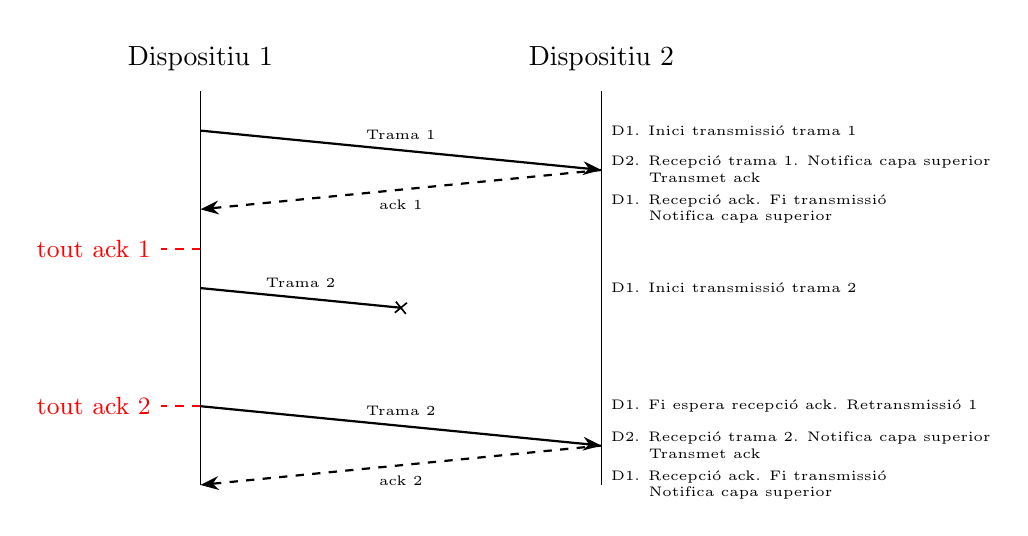
\begin{tikzpicture}[
        device/.style={draw=none, minimum width=1cm, minimum height=0.8cm},
        msg/.style={-Stealth, thick},
        ack/.style={-Stealth, thick, dashed},
        timeout/.style={red, thick, dashed},
        node distance=1cm and 3cm,
        timeline/.style={draw, dashed, white},
        fail/.style={thick, cross at end}
    ]
    
    % Devices
    \node[device] (dev1) at (0,0) {Dispositiu 1};
    \node[device, right=of dev1] (dev2) {Dispositiu 2};
    % \draw[msg] ($dev1.south$) -- ($(dev1.south)+(0,-3)$);
    \draw ($(dev1.south) + (0,0)$) -- ($(dev1.south) + (0,-5)$);
    \draw ($(dev2.south) + (0,0)$) -- ($(dev2.south) + (0,-5)$);
    
    % First message
    \draw[msg] ($(dev1.south)+(0,-0.5)$) -- ($(dev2.south)+(0,-1.0)$) node[midway, above] {\tiny{Trama 1}};
    \draw[ack] ($(dev2.south)+(0,-1.0)$) -- ($(dev1.south)+(0,-1.5)$) node[midway, below] {\tiny{\acro{ack} 1}};
    \draw[timeout] ($(dev1.south)+(0,-2)$) -- ++(-0.5,0) node[left] {\small{\acro{tout ack 1}}};
    \node[right] at ($(dev2.south)+(0,-0.5)$) {\tiny{D1. Inici transmissió trama 1}};
    \node[right] at ($(dev2.south)+(0,-0.9)$) {\tiny{D2. Recepció trama 1. Notifica capa superior}};
    \node[right] at ($(dev2.south)+(0,-1.1)$) {\tiny{\hspace{2em}Transmet \acro{ack}}};
    \node[right] at ($(dev2.south)+(0,-1.4)$) {\tiny{D1. Recepció \acro{ack}. Fi transmissió}};
    \node[right] at ($(dev2.south)+(0,-1.6)$) {\tiny{\hspace{2em}Notifica capa superior}};

    
    % Second message (fails)
    % \draw[fail] ($(dev1.south)+(0,-2.5)$) -- ($(dev2.south)+(0,-3)$) node[midway, above] {\tiny{Trama 2}};
    \draw[fail] ($(dev1.south)+(0,-2.5)$) -- ($ (dev1.south) !0.5! (dev2.south) + (0,-2.75) - (0,0) $) node[midway, above] {\tiny{Trama 2}};
    \draw[timeout] ($(dev1.south)+(0,-4)$) -- ++(-0.5,0) node[left] {\small{\acro{tout ack} 2}};
    \node[right] at ($(dev2.south)+(0,-2.5)$) {\tiny{D1. Inici transmissió trama 2}};
    
    % Retransmit message
    \draw[msg] ($(dev1.south)+(0,-4)$) -- ($(dev2.south)+(0,-4.5)$) node[midway, above] {\tiny{Trama 2}};
    \draw[ack] ($(dev2.south)+(0,-4.5)$) -- ($(dev1.south)+(0,-5)$) node[midway, below] {\tiny{\acro{ack} 2}};
    \node[right] at ($(dev2.south)+(0,-4)$) {\tiny{D1. Fi espera recepció \acro{ack}. Retransmissió 1}};
    \node[right] at ($(dev2.south)+(0,-4.4)$) {\tiny{D2. Recepció trama 2. Notifica capa superior}};
    \node[right] at ($(dev2.south)+(0,-4.6)$) {\tiny{\hspace{2em}Transmet \acro{ack}}};
    \node[right] at ($(dev2.south)+(0,-4.9)$) {\tiny{D1. Recepció \acro{ack}. Fi transmissió}};
    \node[right] at ($(dev2.south)+(0,-5.1)$) {\tiny{\hspace{2em}Notifica capa superior}};

    \end{tikzpicture}
    \caption{Transmissió correcta, i segona transmissió correcta després de reintent.}
    \label{fig:mac_tx_correcte_reintent}
\end{figure}

Una situació més excepcional és la representada a la \autoref{fig:mac_tx_considerat_fallida}, on el dispositiu 1 realitza una transmissió, sense rebre en cap retransmissió el missatge de reconeixement. Malgrat això, el dispositiu 2 sí que havia rebut la trama, generant l'\acro{ack} corresponent, el qual no arriba al dispositiu 1. S'observa com en la segona recepció de la trama, el dispositiu 2 no notifica a la capa superior, ja que ja s'havia processat prèviament. En aquesta situació, el dispositiu 1 considera que la transmissió no ha estat satisfactòria, malgrat que el dispositiu 2 sí que havia rebut la trama.

% TX incorrecte + 3 reintents - Fallada transmissió
\begin{figure}[h]
    \centering
    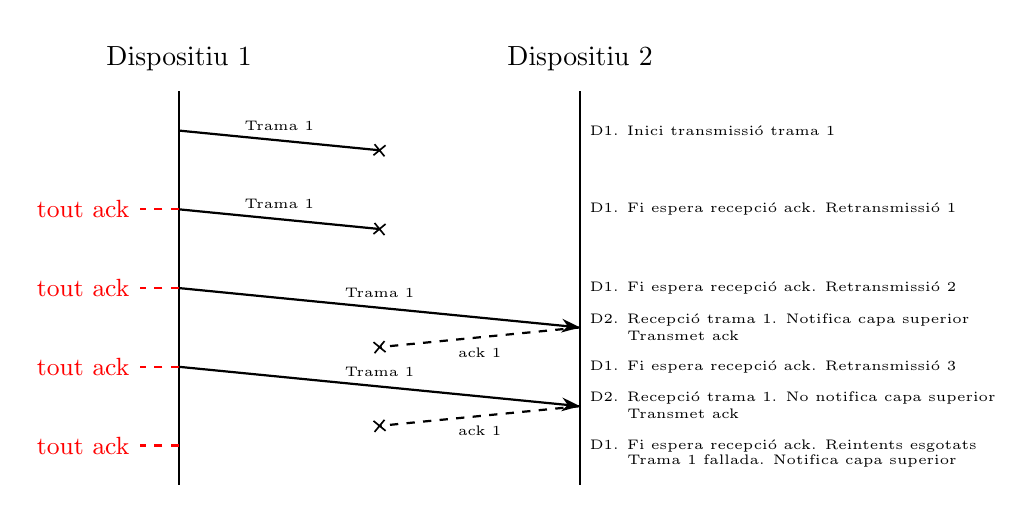
\begin{tikzpicture}[
        node distance=1cm and 3cm,
        device/.style={draw=none, minimum width=1cm, minimum height=0.8cm},
        msg/.style={-Stealth, thick},
        ack/.style={-Stealth, thick, dashed},
        timeout/.style={red, thick, dashed},
        fail/.style={thick, cross at end},
        failAck/.style={thick, cross at end, dashed},
    ]

        % Devices
        \node[device] (dev1) at (0,0) {Dispositiu 1};
        \node[device, right=of dev1] (dev2) {Dispositiu 2};
        % \draw[msg] ($dev1.south$) -- ($(dev1.south)+(0,-3)$);
        \draw ($(dev1.south) + (0,0)$) -- ($(dev1.south) + (0,-5)$);
        \draw ($(dev2.south) + (0,0)$) -- ($(dev2.south) + (0,-5)$);

        % First message
        \draw[fail] ($(dev1.south)+(0,-0.5)$) -- ($ (dev1.south) !0.5! (dev2.south) + (0,-0.75) - (0,0) $) node[midway, above] {\tiny{Trama 1}};
        \draw[timeout] ($(dev1.south)+(0,-1.5)$) -- ++(-0.5,0) node[left] {\small{\acro{tout ack}}};
        \node[right] at ($(dev2.south)+(0,-0.5)$) {\tiny{D1. Inici transmissió trama 1}};
        
        \draw[fail] ($(dev1.south)+(0,-1.5)$) -- ($ (dev1.south) !0.5! (dev2.south) + (0,-1.75) - (0,0) $) node[midway, above] {\tiny{Trama 1}};
        \draw[timeout] ($(dev1.south)+(0,-2.5)$) -- ++(-0.5,0) node[left] {\small{\acro{tout ack}}};
        \node[right] at ($(dev2.south)+(0,-1.5)$) {\tiny{D1. Fi espera recepció \acro{ack}. Retransmissió 1}};

        \draw[msg] ($(dev1.south)+(0,-2.5)$) -- ($ (dev2.south) + (0,-3) $) node[midway, above] {\tiny{Trama 1}};
        \draw[failAck] ($(dev2.south)+(0,-3)$) -- ($(dev1.south) !0.5! (dev2.south)+(0,-3.25)$) node[midway, below] {\tiny{\acro{ack} 1}};
        \draw[timeout] ($(dev1.south)+(0,-3.5)$) -- ++(-0.5,0) node[left] {\small{\acro{tout ack}}};
        \node[right] at ($(dev2.south)+(0,-2.5)$) {\tiny{D1. Fi espera recepció \acro{ack}. Retransmissió 2}};
        \node[right] at ($(dev2.south)+(0,-2.9)$) {\tiny{D2. Recepció trama 1. Notifica capa superior}};
        \node[right] at ($(dev2.south)+(0,-3.1)$) {\tiny{\hspace{2em}Transmet \acro{ack}}};

        % \node[align=left] {\tiny{This is a\\demonstration.}};

        \draw[msg] ($(dev1.south)+(0,-3.5)$) -- ($ (dev2.south) + (0,-4) $) node[midway, above] {\tiny{Trama 1}};
        \draw[failAck] ($(dev2.south)+(0,-4)$) -- ($(dev1.south) !0.5! (dev2.south)+(0,-4.25)$) node[midway, below] {\tiny{\acro{ack} 1}};
        \draw[timeout] ($(dev1.south)+(0,-4.5)$) -- ++(-0.5,0) node[left] {\small{\acro{tout ack}}};
        \node[right] at ($(dev2.south)+(0,-3.5)$) {\tiny{D1. Fi espera recepció \acro{ack}. Retransmissió 3}};
        \node[right] at ($(dev2.south)+(0,-3.9)$) {\tiny{D2. Recepció trama 1. No notifica capa superior}};
        \node[right] at ($(dev2.south)+(0,-4.1)$) {\tiny{\hspace{2em}Transmet \acro{ack}}};

        \node[right] at ($(dev2.south)+(0,-4.5)$) {\tiny{D1. Fi espera recepció \acro{ack}. Reintents esgotats}};
        \node[right] at ($(dev2.south)+(0,-4.7)$) {\tiny{\hspace{2em}Trama 1 fallada. Notifica capa superior}};

    \end{tikzpicture}
    \caption{Transmissió considerada fallida, rebuda correctament per receptor.}
    \label{fig:mac_tx_considerat_fallida}
\end{figure}

Per acabar es mostra una situació més complexa i completa, representada a la \autoref{fig:mac_tx_complet}. Es representen tres dispositius, amb la primera transmissió del dispositiu 2 completada després d'un reintent. En el procés d'espera de recepció de reconeixement, es mostra com aquest rep una trama, enviada pel dispositiu 1, i genera el corresponent \acro{ack}. Per acabar, es representa el comportament de la cua de transmissió, on el dispositiu 2 inicia una nova transmissió just després de rebre el missatge de reconeixement.

\begin{figure}[h]
    \centering
    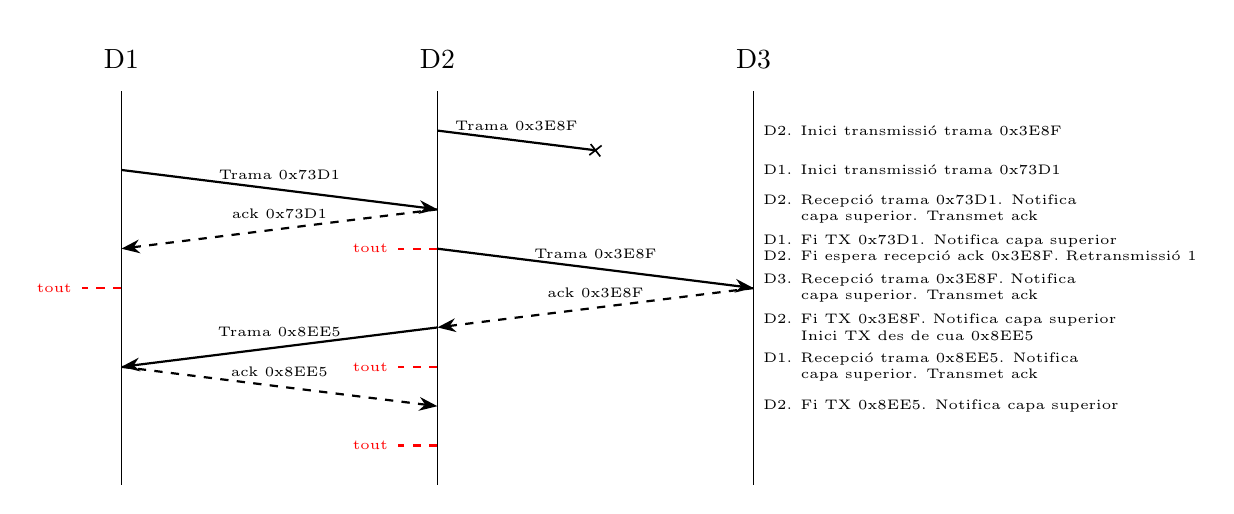
\begin{tikzpicture}[
        node distance=1cm and 3cm,
        device/.style={draw=none, minimum width=1cm, minimum height=0.8cm},
        msg/.style={-Stealth, thick},
        ack/.style={-Stealth, thick, dashed},
        timeout/.style={thick, red, dashed},
        fail/.style={thick, cross at end},
        failAck/.style={thick, cross at end, dashed},
    ]

        % Devices
        \node[device] (dev1) at (0,0) {D1};
        \node[device, right=of dev1] (dev2) {D2};
        \node[device, right=of dev2] (dev3) {D3};
        \draw ($(dev1.south) + (0,0)$) -- ($(dev1.south) + (0,-5)$);
        \draw ($(dev2.south) + (0,0)$) -- ($(dev2.south) + (0,-5)$);
        \draw ($(dev3.south) + (0,0)$) -- ($(dev3.south) + (0,-5)$);

        \draw[fail] ($(dev2.south)+(0,-0.5)$) -- ($ (dev2.south) !0.5! (dev3.south) + (0,-0.75) - (0,0) $) node[midway, above] {\tiny{Trama \fitx{0x3E8F}}};
        \draw[timeout] ($(dev2.south)+(0,-2)$) -- ++(-0.5,0) node[left] {\small{\acro{\tiny{tout}}}};
        \node[right] at ($(dev3.south)+(0,-0.5)$) {\tiny{D2. Inici transmissió trama \fitx{0x3E8F}}};

        \draw[msg] ($(dev1.south)+(0,-1)$) -- ($(dev2.south) + (0,-1.5) - (0,0) $) node[midway, above] {\tiny{Trama \fitx{0x73D1}}};
        \draw[timeout] ($(dev1.south)+(0,-2.5)$) -- ++(-0.5,0) node[left] {\small{\acro{\tiny{tout}}}};
        \node[right] at ($(dev3.south)+(0,-1)$) {\tiny{D1. Inici transmissió trama \fitx{0x73D1}}};

        \draw[ack] ($(dev2.south)+(0,-1.5)$) -- ($(dev1.south)+(0,-2)$) node[midway, above] {\tiny{\acro{ack} \fitx{0x73D1}}};
        \node[right] at ($(dev3.south)+(0,-1.4)$) {\tiny{D2. Recepció trama \fitx{0x73D1}. Notifica}};
        \node[right] at ($(dev3.south)+(0,-1.6)$) {\tiny{\hspace{2em}capa superior. Transmet \acro{ack}}};
        \node[right] at ($(dev3.south)+(0,-1.9)$) {\tiny{D1. Fi TX \fitx{0x73D1}. Notifica capa superior}};
        
        \draw[msg] ($(dev2.south)+(0,-2)$) -- ($(dev3.south) + (0,-2.5) - (0,0) $) node[midway, above] {\tiny{Trama \fitx{0x3E8F}}};
        \draw[ack] ($(dev3.south)+(0,-2.5)$) -- ($(dev2.south)+(0,-3)$) node[midway, above] {\tiny{\acro{ack} \fitx{0x3E8F}}};
        \draw[timeout] ($(dev2.south)+(0,-3.5)$) -- ++(-0.5,0) node[left] {\small{\acro{\tiny{tout}}}};
        \node[right] at ($(dev3.south)+(0,-2.1)$) {\tiny{D2. Fi espera recepció \acro{ack} \fitx{0x3E8F}. Retransmissió 1}};
        \node[right] at ($(dev3.south)+(0,-2.4)$) {\tiny{D3. Recepció trama \fitx{0x3E8F}. Notifica}};
        \node[right] at ($(dev3.south)+(0,-2.6)$) {\tiny{\hspace{2em}capa superior. Transmet \acro{ack}}};

        \draw[msg] ($(dev2.south)+(0,-3)$) -- ($(dev1.south) + (0,-3.5) - (0,0) $) node[midway, above] {\tiny{Trama \fitx{0x8EE5}}};
        \draw[ack] ($(dev1.south)+(0,-3.5)$) -- ($(dev2.south)+(0,-4)$) node[midway, above] {\tiny{\acro{ack} \fitx{0x8EE5}}};
        \draw[timeout] ($(dev2.south)+(0,-4.5)$) -- ++(-0.5,0) node[left] {\small{\acro{\tiny{tout}}}};
        \node[right] at ($(dev3.south)+(0,-2.9)$) {\tiny{D2. Fi TX \fitx{0x3E8F}. Notifica capa superior}};
        \node[right] at ($(dev3.south)+(0,-3.1)$) {\tiny{\hspace{2em}Inici TX des de cua \fitx{0x8EE5}}};
        \node[right] at ($(dev3.south)+(0,-3.4)$) {\tiny{D1. Recepció trama \fitx{0x8EE5}. Notifica}};
        \node[right] at ($(dev3.south)+(0,-3.6)$) {\tiny{\hspace{2em}capa superior. Transmet \acro{ack}}};
        \node[right] at ($(dev3.south)+(0,-4)$) {\tiny{D2. Fi TX \fitx{0x8EE5}. Notifica capa superior}};


    \end{tikzpicture}
    \caption{Transmissió considerada fallida, rebuda correctament per receptor.}
    \label{fig:mac_tx_complet}
\end{figure}

\subsection{Encaminament estàtic}
\subsection{Capa de transport}
\subsection{Capa d’aplicació}
\section{Altres serveis}
\label{sec:altres_serveis}
\subsection{Gestor de tasques}
\section{Proves i validació funcional}

\chapter{Adaptació a entorns de baix consum}
\section{Descripció de l’escenari: xarxa lineal de sensors}
\section{Limitacions del protocol sense optimitzacions energètiques}
% \section{Estratègies de sincronització i activació temporal}
\section{Estratègies de sincronització}
\subsection{Sincronització explícita}
\subsection{Sincronització implícita}
% \subsection{Avantatges i inconvenients de cada enfocament}
% \subsection{Compromisos entre consum i generalitat del protocol}

\chapter{Conclusions}
% \section{Resultats assolits}
% \section{Limitacions del disseny final}
% \section{Punts clau de millora}

\chapter{Treball futur}
% \section{Suport a topologies més complexes}
% \section{Optimització del consum energètic}
% \section{Integració amb LoRaWAN o altres protocols}


% \chapter{Introducció}
% \label{chap:intro}
% \section{Objectius}
% \label{sec:objectius}
% \section{Limitacions del treball}
% \section{Organització de la memòria}

% \chapter{Antecedents}
% \section{Introducció a LoRa i LoRaWAN}
% % Mencionar limitacions legals de TTN i EU868
% \section{Sobre els protocols de comunicació}
% \section{Treballs relacionats}
% % meshtastic -> xarxa mesh però sense baix consum, broadcasts podent afectar communicació, etc.
% % tampoc permeten compatibilitat amb lorawan
% % \section{Solucions existents}
% % loramesher -> sense broadcast, però requereixen descobriment de rutes previs
% % Cap dels dos permeten baix consum i modes de deep sleep

% % Aqui van els capitols especifics del treball
% \chapter{Disseny del protocol de comunicació} % no es veu afectat per material
% \section{Medi físic}
% \subsection{LoRa}
% \subsection{LoRaWAN}
% % Uplinks es faran amb ACK o no depenent de define en compilar
% % fet així per evitar que s'hagin de fer molts downlinks per ACKs
% % ja que TTN limita (fair use policy) a 10 downlinks per dia
% \section{Accés al medi}
% % Mencionar que seria aquí on es faria limitació d'accés al medi
% % Podent afegir un últim estat que "esperi" un temps fins següent TX
% % Parlar llavors sobre les possibles limitacions que això podria comportar
% % (per exemple si es limiten ACKs de capa MAC, o no es limiten, o es limiten ACKs de transport...)
% \section{Encaminament}
% \section{Transport}
% \section{Aplicació}
% \chapter{Implementació del protocol}
% \section{Estructura}
% \subsection{Organització del codi}
% % S'ha implementat seguint model de capes, on cada capa és un mòdul.
% % Cada capa inferior notifica a la superior a través de callbacks, 
% % i cada capa superior notifica a la inferior a través de mètodes.
% % S'ha intentat que no hi hagi mètodes bloquejants, amb excepció dels 
% % mètodes "finals" com transmissió.
% \subsection{Biblioteques i entorn de desenvolupament}
% % platformio + radiolib (comentar radiohead + lmic)
% \section{Protocol de comunicació}
% \subsection{Capa física}
% \subsection{Accés al medi}
% \subsection{Encaminament}
% \subsection{Transport}
% \subsection{Aplicació}
% \section{Validació del funcionament i resultats}

% \chapter{Aplicació en entorns de baix consum}
% % explicar avantatges i inconvenients d'utilitzar
% % el protocol de sincronització genèric aqui. També s'hauria d'explicar el seu disseny

% % quines son totes les opcions plantejades, avantatges i inconvenients, i perquè
% \section{Descripció de la situació}
% % Com és la xarxa, i què es vol aconseguir

% % Per a cada iteració: avantatges i inconvenients. Què implicaria afegir nous nodes?
% % Limitacions de temps? memòria?

% \chapter{Conclusions}

% \chapter{Treball futur}

% https://www.latex-tables.com/
% configurar amb opció de SCALE
\begin{figure}
    \centering
    \resizebox{\linewidth}{!}{%
        \begin{tabular}{l||cccccccccccccccccc} 
            \hhline{~|t|~~~~~~~----~~~~~~~}
            \textbf{N1} &                          &                            &                            &                            &                            &                            & \multicolumn{1}{c|}{}      & \multicolumn{1}{c|}{RX2:9} & \multicolumn{1}{c|}{TX1:9} & \multicolumn{1}{c|}{{\cellcolor[rgb]{0.753,0.749,0.737}}RXG} & \multicolumn{1}{c|}{{\cellcolor[rgb]{0.753,0.749,0.737}}TXG} &                                                              &                                                              &                          &                          &                          &                          &                           \\ 
            \hhline{~||~~~~~~------~~~~~~}
            \textbf{N2} &                          &                            &                            &                            &                            & \multicolumn{1}{c|}{}      & \multicolumn{1}{c|}{RX3:9} & \multicolumn{1}{c|}{TX2:9} &                            & \multicolumn{1}{c|}{}                                        & \multicolumn{1}{c|}{{\cellcolor[rgb]{0.753,0.749,0.737}}RXG} & \multicolumn{1}{c|}{{\cellcolor[rgb]{0.753,0.749,0.737}}TXG} &                                                              &                          &                          &                          &                          &                           \\ 
            \hhline{~||~~~~~---~~---~~~~~}
            \textbf{N3} &                          &                            &                            &                            & \multicolumn{1}{c|}{}      & \multicolumn{1}{c|}{RX4:9} & \multicolumn{1}{c|}{TX3:9} &                            &                            &                                                              & \multicolumn{1}{c|}{}                                        & \multicolumn{1}{c|}{{\cellcolor[rgb]{0.753,0.749,0.737}}RXG} & \multicolumn{1}{c|}{{\cellcolor[rgb]{0.753,0.749,0.737}}TXG} &                          &                          &                          &                          &                           \\ 
            \hhline{~||~~~~---~~~~---~~~~}
            \textbf{N4} &                          &                            &                            & \multicolumn{1}{c|}{}      & \multicolumn{1}{c|}{RX5:9} & \multicolumn{1}{c|}{TX4:9} &                            &                            &                            &                                                              &                                                              & \multicolumn{1}{c|}{}                                        & \multicolumn{1}{c|}{{\cellcolor[rgb]{0.753,0.749,0.737}}RXG} & \multicolumn{1}{c|}{TXG} &                          &                          &                          &                           \\ 
            \cline{5-7}\cline{14-16}
            \textbf{N5} &                          &                            & \multicolumn{1}{c|}{}      & \multicolumn{1}{c|}{RX6:9} & \multicolumn{1}{c|}{TX5:9} &                            &                            &                            &                            &                                                              &                                                              &                                                              & \multicolumn{1}{c|}{}                                        & \multicolumn{1}{c|}{RXG} & \multicolumn{1}{c|}{TXG} &                          &                          &                           \\ 
            \cline{4-6}\cline{15-17}
            \textbf{N6} &                          & \multicolumn{1}{c|}{}      & \multicolumn{1}{c|}{RX7:9} & \multicolumn{1}{c|}{TX6:9} &                            &                            &                            &                            &                            &                                                              &                                                              &                                                              &                                                              & \multicolumn{1}{c|}{}    & \multicolumn{1}{c|}{RXG} & \multicolumn{1}{c|}{TXG} &                          &                           \\ 
            \cline{3-5}\cline{16-18}
            \textbf{N7} & \multicolumn{1}{c|}{}    & \multicolumn{1}{c|}{RX8:9} & \multicolumn{1}{c|}{TX7:9} &                            &                            &                            &                            &                            &                            &                                                              &                                                              &                                                              &                                                              &                          & \multicolumn{1}{c|}{}    & \multicolumn{1}{c|}{RXG} & \multicolumn{1}{c|}{TXG} &                           \\ 
            \cline{2-4}\cline{17-19}
            \textbf{N8} & \multicolumn{1}{c|}{RX9} & \multicolumn{1}{c|}{TX8:9} &                            &                            &                            &                            &                            &                            &                            &                                                              &                                                              &                                                              &                                                              &                          &                          & \multicolumn{1}{c|}{}    & \multicolumn{1}{c|}{RXG} & \multicolumn{1}{c|}{TXG}  \\ 
            \cline{2-3}\cline{18-19}
            \textcolor[rgb]{0.1,1,0.2}{\textbf{N9}} & \multicolumn{1}{c|}{TX9} &                            &                            &                            &                            &                            &                            &                            &                            &                                                              &                                                              &                                                              &                                                              &                          &                          &                          & \multicolumn{1}{c|}{}    & \multicolumn{1}{c|}{RXG}  \\
            \cline{2-2}\cline{19-19}
        \end{tabular}
    }
    \caption{Model sense missatge de sincronització, amb dades acumulatives}
    \label{fig:noSyncAcumulatiu}
\end{figure}

\listoftables
\listoffigures

\printbibliography


% Si feu servir apèndixs, descomenteu
% (també la  \part del principi del document)
%\appendix
%\part{Apèndixs}
%\chapter{Un apèndix}


% ABANS D'ENTREGAR MIRAR QUE L·L ESTIGUIN BEN ESCRITES AMB \l.l

\end{document}

%%% Local Variables:
%%% mode: latex
%%% TeX-master: t
%%% LaTeX-biblatex-use-Biber: t
%%% End:
